% SAIM blog-post entrypoint (pdfLaTeX). Template v1.2.
\documentclass[numbered]{saim-blog}
% SAIM metadata registry. Do not edit during normal use.
%
% Edit the document identity in project.tex and the people in people.tex
% (both at the project root). This file only implements the registry and
% derives every display, plain-text, bibliography, and PDF string from them.
%
% People syntax (people.tex):
%   \Affiliation{key}{Institution name}
%   \Author{Name}{email}{affiliation-key-list}
%   \CorrespondingAuthor{Name}{email}  % optional override
%
% The author line carries that author's email and one or more affiliation keys.
% Multiple authors can reuse the same affiliation key. Do not edit author,
% affiliation, or email lists anywhere else.

% Post identity: edit this block for each new post.
\newcommand{\ProjectTitle}{A Statistical Assessment of ``War May Answer Longtime Riddle of Iranian Dams Built for No Clear Reason''}
\newcommand{\ProjectShortTitle}{Statistical assessment of the NYT Iranian dams article}
\newcommand{\ProjectSubtitle}{\emph{The New York Times}, 16 November 2026}
\newcommand{\ProjectSeriesLabel}{SAIM NOTES}          % series eyebrow
\def\ProjectIssue{}                                   % empty hides (\def, so the class \ifx test sees it as empty)
\newcommand{\ProjectReadingTime}{15 min read}            % leave empty to hide
\newcommand{\ProjectTags}{statistics, spatial analysis, Iran, water, dams}  % comma list; empty hides
\newcommand{\ProjectDate}{17 November 2026}
\newcommand{\ProjectVersion}{v1.0}
\newcommand{\ProjectKeywords}{Iran, dams, missile bases, spatial statistics, point patterns, international humanitarian law}
% Author card (end of post). Leave either empty to hide it.
\newcommand{\ProjectAuthorBio}{Statistician and AI research scientist.}
\newcommand{\ProjectLinks}{\href{https://github.com/osolari/iran-dams-colocation}{github.com/osolari/iran-dams-colocation}\enspace\textcolor{RuleDark}{\textbullet}\enspace
\href{https://osolari.github.io/iran-dams-colocation}{osolari.github.io/iran-dams-colocation}}


% ---------------------------------------------------------------------------
% Registry implementation. Do not edit this section during normal use.
% ---------------------------------------------------------------------------
\makeatletter
\newcounter{AuthorCounter}
\newcounter{AffiliationCounter}

\newcommand{\ProjectMetaSep}{\enspace\textbullet\enspace}
\newcommand{\ProjectWhiteMetaSep}{\enspace\textbullet\enspace}
% Affiliation superscripts are typeset only when more than one affiliation
% is declared; a single-affiliation project shows clean names.
\newcommand{\AuthorEntry}[2]{#1\ifnum\value{AffiliationCounter}>1\relax\textsuperscript{#2}\fi}
\newcommand{\AffiliationEntry}[2]{\ifnum\value{AffiliationCounter}>1\relax\textsuperscript{#1}\fi#2}

\newcommand{\AuthorListTypeset}{}
\newcommand{\AuthorListPlain}{}
\newcommand{\AuthorListPDF}{}
\newcommand{\AuthorListBib}{}
\newcommand{\AffiliationListTypeset}{}
\newcommand{\AffiliationListPlain}{}
\newcommand{\AffiliationListPDF}{}
\newcommand{\EmailListTypeset}{}
\newcommand{\EmailListPlain}{}
\newcommand{\EmailListPDF}{}
\newcommand{\AuthorEmailListTypeset}{}
\newcommand{\AuthorEmailListPlain}{}
\newcommand{\AuthorEmailListPDF}{}
\newcommand{\LeadAuthor}{}
\newcommand{\LeadAuthorEmail}{}
\newcommand{\CorrespondingAuthorName}{}
\newcommand{\CorrespondenceEmail}{}

\newcommand{\ResetPeople}{%
  \setcounter{AuthorCounter}{0}%
  \setcounter{AffiliationCounter}{0}%
  \gdef\AuthorListTypeset{}%
  \gdef\AuthorListPlain{}%
  \gdef\AuthorListPDF{}%
  \gdef\AuthorListBib{}%
  \gdef\AffiliationListTypeset{}%
  \gdef\AffiliationListPlain{}%
  \gdef\AffiliationListPDF{}%
  \gdef\EmailListTypeset{}%
  \gdef\EmailListPlain{}%
  \gdef\EmailListPDF{}%
  \gdef\AuthorEmailListTypeset{}%
  \gdef\AuthorEmailListPlain{}%
  \gdef\AuthorEmailListPDF{}%
  \gdef\LeadAuthor{}%
  \gdef\LeadAuthorEmail{}%
  \gdef\CorrespondingAuthorName{}%
  \gdef\CorrespondenceEmail{}%
}

% Declare one unique affiliation. The first argument is the key used by authors.
% Example: \Affiliation{saim}{sAIm Labs}
\newcommand{\Affiliation}[2]{%
  \stepcounter{AffiliationCounter}%
  \expandafter\xdef\csname AffiliationMark@#1\endcsname{\arabic{AffiliationCounter}}%
  \expandafter\gdef\csname AffiliationText@#1\endcsname{#2}%
  \ifnum\value{AffiliationCounter}>1\relax
    \g@addto@macro\AffiliationListTypeset{\ProjectMetaSep}%
    \g@addto@macro\AffiliationListPlain{\ProjectMetaSep}%
    \g@addto@macro\AffiliationListPDF{; }%
  \fi
  \g@addto@macro\AffiliationListTypeset{\AffiliationEntry{\csname AffiliationMark@#1\endcsname}{#2}}%
  \g@addto@macro\AffiliationListPlain{#2}%
  \g@addto@macro\AffiliationListPDF{\csname AffiliationMark@#1\endcsname: #2}%
}

\ExplSyntaxOn
\cs_new_protected:Npn \saim_unknown_affiliation:n #1
  {
    \PackageError{saim-metadata}{Unknown affiliation key `#1'}
      {Declare it first with \string\Affiliation{#1}{Institution name}.}
  }
\cs_new:Npn \saim_affiliation_mark:n #1
  {
    \cs_if_exist_use:cF { AffiliationMark@\tl_trim_spaces:n {#1} }
      { \saim_unknown_affiliation:n {#1} }
  }
\int_new:N \l_saim_affiliation_mark_index_int
\cs_new:Npn \saim_affiliation_marks:n #1
  {
    \int_zero:N \l_saim_affiliation_mark_index_int
    \clist_map_inline:nn {#1}
      {
        \int_incr:N \l_saim_affiliation_mark_index_int
        \int_compare:nNnT {\l_saim_affiliation_mark_index_int} > {1} {,}%
        \saim_affiliation_mark:n {##1}
      }
  }
\NewDocumentCommand{\AffiliationMarks}{m}{\saim_affiliation_marks:n {#1}}
\ExplSyntaxOff

% Declare one author. The third argument is a comma-separated list of affiliation keys.
% Example: \Author{Ada Lovelace}{ada@example.com}{saim,exampleu}
\newcommand{\Author}[3]{%
  \stepcounter{AuthorCounter}%
  \ifnum\value{AuthorCounter}=1\relax
    \gdef\LeadAuthor{#1}%
    \gdef\LeadAuthorEmail{#2}%
    \gdef\CorrespondingAuthorName{#1}%
    \gdef\CorrespondenceEmail{#2}%
  \else
    \g@addto@macro\AuthorListTypeset{\ProjectMetaSep}%
    \g@addto@macro\AuthorListPlain{\ProjectMetaSep}%
    \g@addto@macro\AuthorListPDF{; }%
    \g@addto@macro\AuthorListBib{\ and }%
  \fi
  \g@addto@macro\AuthorListTypeset{\AuthorEntry{#1}{\AffiliationMarks{#3}}}%
  \g@addto@macro\AuthorListPlain{#1}%
  \g@addto@macro\AuthorListPDF{#1}%
  \g@addto@macro\AuthorListBib{#1}%
  \if\relax\detokenize{#2}\relax\else
    \ifx\EmailListPlain\@empty\else
      \g@addto@macro\EmailListTypeset{\ProjectMetaSep}%
      \g@addto@macro\EmailListPlain{\ProjectMetaSep}%
      \g@addto@macro\EmailListPDF{; }%
      \g@addto@macro\AuthorEmailListTypeset{\ProjectMetaSep}%
      \g@addto@macro\AuthorEmailListPlain{\ProjectMetaSep}%
      \g@addto@macro\AuthorEmailListPDF{; }%
    \fi
    \g@addto@macro\EmailListTypeset{\href{mailto:#2}{\nolinkurl{#2}}}%
    \g@addto@macro\EmailListPlain{#2}%
    \g@addto@macro\EmailListPDF{#2}%
    \g@addto@macro\AuthorEmailListTypeset{#1\enspace\href{mailto:#2}{\texttt{<#2>}}}%
    \g@addto@macro\AuthorEmailListPlain{#1\enspace\textless#2\textgreater}%
    \g@addto@macro\AuthorEmailListPDF{#1 <#2>}%
  \fi
}

% Optional override: correspondence defaults to the first author, but this
% declaration lets author order and correspondence remain independent.
\newcommand{\CorrespondingAuthor}[2]{%
  \gdef\CorrespondingAuthorName{#1}%
  \gdef\CorrespondenceEmail{#2}%
}

% Optional descriptive aliases; normal users can ignore these.
\let\DeclareAffiliation\Affiliation
\let\DeclareAuthor\Author
\makeatother

% ---------------------------------------------------------------------------
% Derived display macros consumed by all targets.
% ---------------------------------------------------------------------------
\newcommand{\ProjectAuthorsDisplay}{\texorpdfstring{\AuthorListTypeset}{\AuthorListPDF}}
\newcommand{\ProjectAuthorsPlainDisplay}{\AuthorListPlain}
\newcommand{\ProjectAuthorsPDF}{\AuthorListPDF}
\newcommand{\ProjectAuthorsBib}{\AuthorListBib}
\newcommand{\ProjectAffiliationsDisplay}{\texorpdfstring{\AffiliationListTypeset}{\AffiliationListPDF}}
\newcommand{\ProjectAffiliationsPlainDisplay}{\AffiliationListPlain}
\newcommand{\ProjectAffiliationsPDF}{\AffiliationListPDF}
\newcommand{\ProjectEmailsDisplay}{\texorpdfstring{\EmailListTypeset}{\EmailListPDF}}
\newcommand{\ProjectEmailsPlainDisplay}{\EmailListPlain}
\newcommand{\ProjectEmailsPDF}{\EmailListPDF}
\newcommand{\ProjectAuthorEmailsDisplay}{\texorpdfstring{\AuthorEmailListTypeset}{\AuthorEmailListPDF}}
\newcommand{\ProjectAuthorEmailsPlainDisplay}{\AuthorEmailListPlain}
\newcommand{\ProjectAuthorEmailsPDF}{\AuthorEmailListPDF}
\newcommand{\ProjectLeadAuthor}{\LeadAuthor}
\newcommand{\ProjectLeadAuthorEmail}{\LeadAuthorEmail}
\newcommand{\ProjectCorrespondingAuthor}{\CorrespondingAuthorName}
\newcommand{\ProjectCorrespondence}{\CorrespondenceEmail}
\newcommand{\ProjectContactDisplay}{\ProjectEmailsDisplay}

% ---------------------------------------------------------------------------
% People declarations. Edit people.tex for authors, emails, affiliations,
% and (optionally) the corresponding-author override.
% ---------------------------------------------------------------------------
% People: edit this file once for all authors, affiliations, and emails.
%
%   \Affiliation{key}{Institution name}          declare each affiliation once
%   \Author{Name}{email}{key1,key2}              declare each author once
%   \CorrespondingAuthor{Name}{email}            optional; defaults to first author

\ResetPeople

\Affiliation{ucb}{Ph.D.\ in Statistics, University of California, Berkeley}
\Affiliation{saim}{sAIm Labs}

\Author{Omid S.\ Solari, Ph.D.}{}{ucb,saim}


% ---------------------------------------------------------------------------
% Target metadata appliers. Target files call these; they do not hard-code
% people metadata.
% ---------------------------------------------------------------------------
\newcommand{\DeclareProjectPaperPeople}{%
  \gdef\authorlist{\ProjectAuthorsDisplay}%
  \gdef\affiliationlist{\ProjectAffiliationsDisplay}%
}
\newcommand{\DeclareProjectPaperAuthors}{\DeclareProjectPaperPeople}
\newcommand{\DeclareProjectPaperAffiliations}{\DeclareProjectPaperPeople}

\makeatletter
\newcommand{\ProjectMaybeAddEmailMetadata}{%
  \ifx\EmailListPlain\@empty\else
    \metadata[Emails]{\ProjectContactDisplay}%
  \fi
}
\makeatother

\newcommand{\ApplyProjectSlideMetadata}{%
  \title[\ProjectShortTitle]{\ProjectTitle}%
  \subtitle{\ProjectSubtitle}%
  \author{\ProjectAuthorsDisplay}%
  \institute{\ProjectAffiliationsDisplay}%
  \date{\ProjectDate}%
}


\graphicspath{{figures/}{shared/brand/logos/}}
% =============================================================================
% math.tex - shared project notation
% =============================================================================
% Do not load packages here. The document entrypoints load amsmath, amssymb,
% amsfonts, amsthm, mathtools, and any project-specific dependencies.

% Number sets and expectations
\providecommand{\R}{\mathbb{R}}
\providecommand{\E}{\mathbb{E}}

% Common operators
\providecommand{\KL}{\operatorname{KL}}
\providecommand{\DKL}{D_{\mathrm{KL}}}
\providecommand{\Var}{\operatorname{Var}}
\providecommand{\Cov}{\operatorname{Cov}}
\providecommand{\argmax}{\operatorname*{arg\,max}}
\providecommand{\argmin}{\operatorname*{arg\,min}}

% Delimiters
\providecommand{\norm}[1]{\left\lVert #1 \right\rVert}
\providecommand{\abs}[1]{\left\lvert #1 \right\rvert}
\providecommand{\set}[1]{\left\{ #1 \right\}}
\providecommand{\paren}[1]{\left( #1 \right)}
\providecommand{\bracket}[1]{\left[ #1 \right]}
\providecommand{\ip}[2]{\left\langle #1, #2 \right\rangle}

% Example policy notation. Delete or extend for a different project.
\providecommand{\pitheta}{\pi_{\theta}}
\providecommand{\piref}{\pi_{\mathrm{ref}}}
\providecommand{\pistar}{\pi^{*}}

\usepackage{longtable}
\usepackage{xurl}
\renewcommand{\bibfont}{\small\RaggedRight}
% auto-generated by src/make_tex.py; do not edit
\newcommand{\NBases}{25}
\newcommand{\NDams}{183}
\newcommand{\NLargeDams}{66}
\newcommand{\NSim}{10,000}
\newcommand{\ObsMedian}{48.1}
\newcommand{\ObsMean}{57.5}
\newcommand{\ObsShareTen}{8}
\newcommand{\ObsShareTwenty}{12}
\newcommand{\NullCSR}{62.3}
\newcommand{\PCSR}{0.146}
\newcommand{\RatioCSR}{0.77}
\newcommand{\NullMOne}{60.3}
\newcommand{\PMOne}{0.151}
\newcommand{\RatioMOne}{0.80}
\newcommand{\NullMTwo}{44.2}
\newcommand{\PMTwo}{0.689}
\newcommand{\RatioMTwo}{1.09}
\newcommand{\NullMThree}{39.6}
\newcommand{\PMThree}{0.908}
\newcommand{\RatioMThree}{1.21}
\newcommand{\NullRIV}{35.3}
\newcommand{\PRIV}{0.963}
\newcommand{\RatioRIV}{1.36}
\newcommand{\PLargeCSR}{0.131}
\newcommand{\PLargeMThree}{0.725}
\newcommand{\MedStruck}{48.1}
\newcommand{\MedNotStruck}{56.9}
\newcommand{\PStruck}{0.30}
\newcommand{\CityObs}{35.7}
\newcommand{\CityPCSR}{$<$0.001}
\newcommand{\CityPM}{0.506}
\newcommand{\AirObs}{47.6}
\newcommand{\AirPCSR}{0.052}
\newcommand{\AirPM}{0.856}
\newcommand{\DamsNear}{9}
\newcommand{\YearNear}{2008}
\newcommand{\YearFar}{2009}
\newcommand{\PYear}{0.99}
\newcommand{\BaseCity}{44.8}
\newcommand{\IranCity}{92.5}
\newcommand{\BaseRiver}{15.2}
\newcommand{\IranRiver}{33.4}
\newcommand{\PMeanCSR}{0.011}
\newcommand{\PMeanMThreeMin}{0.454}
\newcommand{\GBases}{5,806}
\newcommand{\GCountries}{53}
\newcommand{\GIranWD}{22}
\newcommand{\AlmaWater}{44.5}
\newcommand{\AlmaDam}{48.1}
\newcommand{\AlmaCoast}{239.8}
\newcommand{\AlmaWaterRatio}{0.81}
\newcommand{\RankWater}{49}
\newcommand{\RankOf}{54}
\newcommand{\RankDam}{45}
\newcommand{\RankWaterRatio}{47}
\newcommand{\RankDamRatio}{29}
\newcommand{\ShareCloser}{91}
\newcommand{\IranTLpeak}{2015}
\newcommand{\IranTLmed}{2009}
\newcommand{\TurTLpeak}{2015}
\newcommand{\IranAfterNinety}{89}
\newcommand{\TurAfterNinety}{79}

\makeatletter\newcommand{\inputtable}[1]{\@@input #1 }\makeatother

% Show the affiliations on their own line under the author in the opening.
\makeatletter
\patchcmd{\maketitle}{\textbf{\color{Ink}\ProjectAuthorsPlainDisplay}%
   \saimblogsep{\color{Muted}\ProjectDate}}{\textbf{\color{Ink}\ProjectAuthorsPlainDisplay}\par
   {\color{Muted}\ProjectAffiliationsPlainDisplay}\par
   {\color{Muted}\ProjectDate}}{}{\PackageError{main}{Could not patch maketitle byline}{}}
\makeatother

\hypersetup{
  pdftitle={A Statistical Assessment of "War May Answer Longtime Riddle of Iranian Dams Built for No Clear Reason"},
  pdfauthor={\ProjectAuthorsPDF},
  pdfsubject={The New York Times, 16 November 2026},
  pdfkeywords={\ProjectKeywords}
}

\begin{document}
\maketitle

\begin{tldr}[Abstract]
\setlength{\parskip}{0.55em}
On 16 November 2026 \emph{The New York Times} (NYT) suggested that Iran built an unusually large number of dams to supply its underground missile sites, pointing to a geographic overlap between dams and the sites struck by the United States and Israel \citep{nyt2026dams}. We tested this claim with open data.\footnote{All code, data and figures: \url{https://github.com/osolari/iran-dams-colocation}. Documentation: \url{https://osolari.github.io/iran-dams-colocation}.} \textbf{The data do not support it.}

\textbf{First, there is no unusual overlap between dams and missile bases.} The \NBases{} medium-range launch bases lie a median of \ObsMedian{}~km from the nearest of Iran's \NDams{} mapped dams, \textbf{not significantly closer than random locations in Iran} ($p=\PCSR$). A small difference in mean distance ($p=\PMeanCSR$) disappears once bases are compared with locations of similar terrain and similar distance to towns and rivers; \textbf{against those locations the bases are farther from dams than expected} ($p=\PMThree$). \textbf{Iranian towns and airports show the same apparent overlap with dams, and towns show more of it.} The overlap reflects where people live and where rivers run, not military design.

\textbf{Second, military bases near water are the norm, not the exception.} Compared with military sites in \GCountries{} other states, \textbf{Iran's launch bases rank \RankWater{}th of \RankOf{} for proximity to a dam or the coast: military sites in \ShareCloser\% of these states lie closer to water.}

\textbf{Third, Iran's dam numbers are not unusual for a water-scarce country.} \textbf{Its dam density is lower than that of Spain, Turkey or Morocco}, and its construction boom followed the same timeline as Turkey's.

\textbf{The NYT article's claim that Iran's dams were built to serve its missile programme is therefore not supported by the evidence.}
\end{tldr}

\section{The NYT article's claims}
As reported in syndicated excerpts \citep{nyt2026dams,moa2026}, the NYT article makes three connected claims:
\begin{enumerate}
\item Iran has an unusually large number of dams (at least 533, ``among the most of any country in the region''), many in places with no apparent civilian need.
\item A map of airstrikes on suspected missile sites ``nearly matched'' a map of those dams.
\item The dams may therefore have been built to supply water and power to hardened military sites. The NYT authors describe this inference as ``speculative'' but ``highly suggestive''.
\end{enumerate}
The second claim concerns spatial co-location and can be tested directly. The first is comparative and can be assessed against other countries. The third is causal: location data can weaken it, if the first two claims fail, but cannot establish or exclude it. Section~\ref{sec:law} sets out why the NYT article's framing of Iran's dams as military infrastructure has legal consequences.

\section{Data}
\begin{center}
\small
\begin{tabularx}{\linewidth}{@{}>{\RaggedRight}p{2.5cm}>{\RaggedRight}X>{\RaggedRight}p{3.4cm}@{}}
\toprule
Layer & Content & Source \\
\midrule
Dams (Iran and global) & 41,145 barriers worldwide; \NDams{} in Iran, of which \NLargeDams{} are large (GRanD-derived) & Global Dam Watch v1.0 \citep{lehner2024gdw,lehner2011grand} \\
Missile launch bases & \NBases{} medium-range launch bases with coordinates; 19 struck in June 2025, 6 not attacked & \citet{alma2026} \\
Military sites worldwide & \GBases{} current sites in \GCountries{} countries with at least 15 sites & \citet{wikidata} \\
Terrain & Elevation and local relief on a 10 arc-minute grid & ETOPO1 \citep{amante2009etopo1} \\
Rivers, settlements, airports & Iranian river network and airports; towns of at least 50,000 & \citet{globalmapiran,naturalearth} \\
Coastline, borders & 1:10m coastline (including the Caspian) and national boundaries & \citet{naturalearth} \\
\bottomrule
\end{tabularx}
\end{center}
Two inputs used by the NYT article are not public. The first is Nima Shokri's map of 533 Iranian dams. In its place we use Global Dam Watch (GDW), the standard harmonised global database, which records \NDams{} Iranian dams, roughly a third of that number. A more complete dam inventory would shorten distances for every type of site, not only for missile bases; because each test below compares the 25 launch bases with matched sites under the same inventory, omitted small dams affect both sides of the comparison. The second is the NYT article's map of 2026 strikes. In its place we use the Alma Research Center's list of the 25 principal medium-range launch bases, 19 of which were struck in June 2025. We could not assess how far the Alma list overlaps with the NYT article's 2026 strike map. The analysis can be rerun directly if either layer is released.

\section{Is the overlap unusual?}
\label{sec:test}
\subsection{Method}
For each base we compute the great-circle distance to the nearest dam and summarise the 25 distances by their median (the primary statistic), their mean and the share within 20~km. We then estimate how often comparison sites, drawn \NSim{} times, are at least as close. The comparison sites come from a sequence of null models of increasing stringency:
\begin{description}
\item[CSR] locations drawn uniformly at random within Iran. This is the comparison implicit in a visual reading of two maps.
\item[M1] for each base, a random location among the 40 grid cells closest to it in elevation and local relief.
\item[M2] as M1, additionally matched on distance to the nearest town of at least 50,000 inhabitants.
\item[M3] as M2, additionally matched on distance to the nearest mapped river.
\item[RIV] the bases are held fixed and the \NDams{} dams are relocated at random along Iran's river network.
\end{description}
Sampled locations are jittered uniformly within their 10$'$ cell. All $p$-values are one-sided, testing whether the bases are closer to dams than expected.

\subsection{Results}
\begin{figure}[t]
\centering
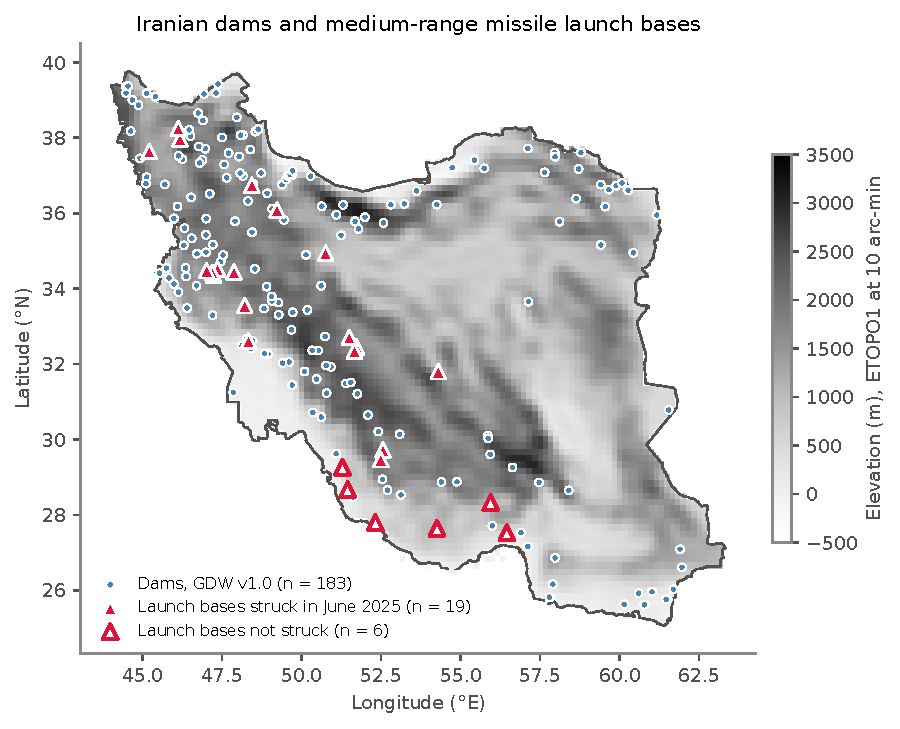
\includegraphics[width=\linewidth]{figures/fig1_map.pdf}
\caption{Iranian dams (GDW v1.0) and the 25 medium-range launch bases catalogued by \citet{alma2026}. Both are concentrated along the populated Zagros and Alborz arc, where towns, rivers and roads are also concentrated.}
\label{fig:map}
\end{figure}

\begin{table}[h]
\centering\small
\begin{tabularx}{\linewidth}{@{}>{\RaggedRight}Xcccc@{}}
\toprule
Null model & Expected (km) & 95\% range & Obs./exp. & $p$ \\
\midrule
\inputtable{tab_nulls.tex}
\bottomrule
\end{tabularx}
\caption{Observed median base-to-dam distance (\ObsMedian{}~km) compared with each null model (\NSim{} simulations). Expected = median of the simulated medians; $p$ is one-sided.}
\label{tab:nulls}
\end{table}

\begin{figure}[t]
\centering
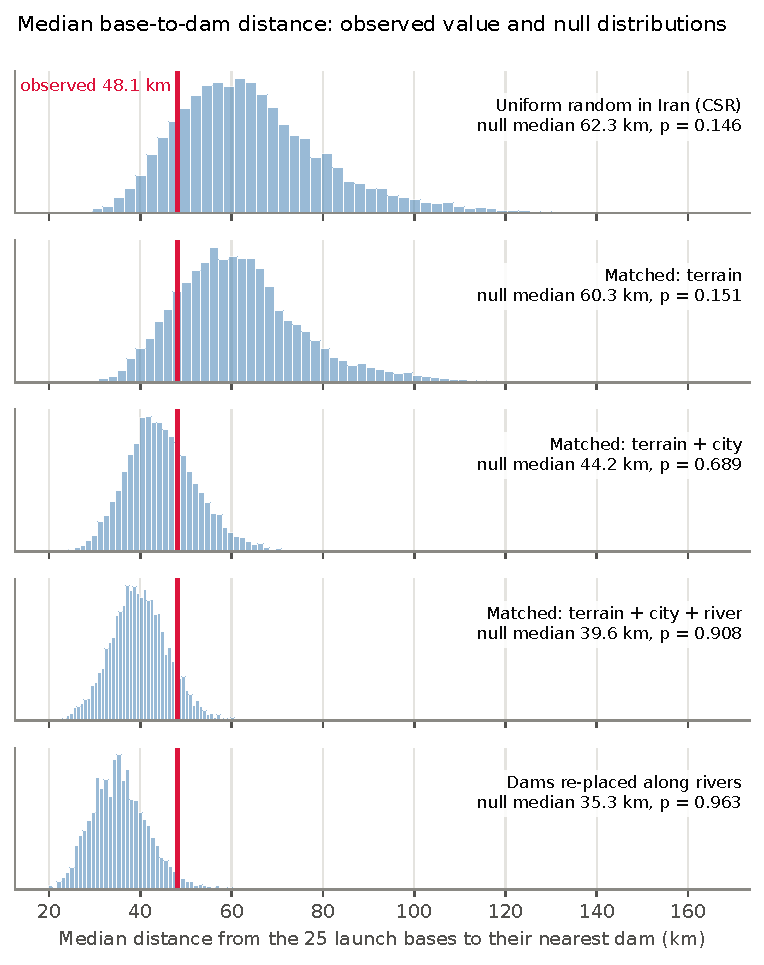
\includegraphics[width=\linewidth]{figures/fig2_nulls.pdf}
\caption{Simulated distributions of the median base-to-dam distance under each null model. The vertical line marks the observed value.}
\label{fig:nulls}
\end{figure}

The results are summarised in Table~\ref{tab:nulls} and Figures~\ref{fig:nulls} and~\ref{fig:ecdf}.

\textbf{The unadjusted association is weak.} Only \ObsShareTen\% of bases lie within 10~km of a dam, and \ObsShareTwenty\% within 20~km. Relative to random locations in Iran, the median distance is not significantly smaller ($p=\PCSR$). The mean distance is significantly smaller ($p=\PMeanCSR$), indicating a modest tendency for bases to lie closer to dams than an arbitrary point in Iran, much of which is desert.

\textbf{The association is explained by settlement geography.} The bases lie on average \BaseCity{}~km from a town of at least 50,000 and \BaseRiver{}~km from a river, compared with \IranCity{}~km and \IranRiver{}~km for Iran as a whole. Dams occupy the same river valleys that supply those towns. Matching on terrain alone leaves the association in place (M1, $p=\PMOne$). Adding distance to towns and rivers removes it: the bases then lie \emph{farther} from dams than their matched comparisons (M3, observed/expected $=\RatioMThree$, $p=\PMThree$). For the mean, $p\ge\PMeanMThreeMin$ across all match sizes (Table~\ref{tab:sens}).

\textbf{Placebo sites show the same pattern.} Iranian towns of at least 50,000 lie a median of \CityObs{}~km from a dam, closer than the missile bases, and the difference from random locations is highly significant ($p=\CityPCSR$). Airports give a similar result ($p=\AirPCSR$). Under the matched null neither is unusual ($p=\CityPM$ and $p=\AirPM$; Figure~\ref{fig:placebo}). The overlap described in the NYT article is therefore what one would expect of any infrastructure in western and central Iran.

\begin{figure}[t]
\centering
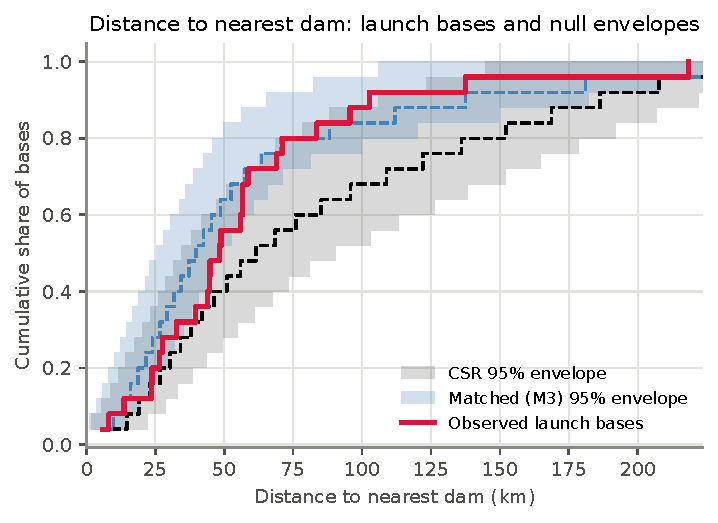
\includegraphics[width=\linewidth]{figures/fig3_ecdf.pdf}
\caption{Empirical cumulative distribution of base-to-dam distances, with 95\% envelopes under CSR and under the fully matched null M3.}
\label{fig:ecdf}
\end{figure}

\begin{figure}[t]
\centering
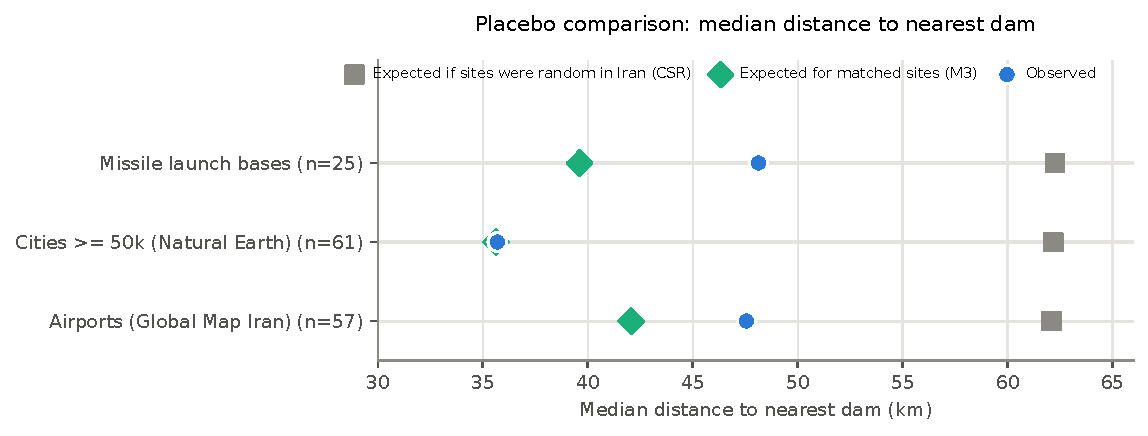
\includegraphics[width=\linewidth]{figures/fig4_placebo.pdf}
\caption{Placebo comparison. Under the unadjusted test, towns and airports appear at least as close to dams as the missile bases; none is unusual once sites are matched.}
\label{fig:placebo}
\end{figure}

\paragraph{Robustness.}
Restricting the analysis to the \NLargeDams{} large dams yields the same conclusion (CSR $p=\PLargeCSR$; M3 $p=\PLargeMThree$). Bases struck in June 2025 are no closer to dams than those that were not attacked (medians \MedStruck{} and \MedNotStruck{}~km; Mann--Whitney $p=\PStruck$). If dams had been built to serve the bases, dams near bases might be expected to differ from the remainder. The \DamsNear{} dams within 25~km of a base have a median completion year of \YearNear{}, compared with \YearFar{} for all other dams ($p=\PYear$), and their recorded uses (irrigation, hydropower and flood control) are typical of the civilian inventory.

\begin{table}[h]
\centering\small
\begin{tabular}{@{}llccc@{}}
\toprule
Null & Match size $k$ & Median & Mean & Share within 20 km \\
\midrule
\inputtable{tab_sensitivity.tex}
\bottomrule
\end{tabular}
\caption{One-sided $p$-values by test statistic and match size (3,000 simulations each).}
\label{tab:sens}
\end{table}

\section{Proximity of military installations to water}
\label{sec:global}
The NYT article presents the proximity of military sites to water infrastructure as anomalous. Historically, military installations have been sited near water for drinking supply, cooling, power and logistics. The United States chose Hanford for its plutonium reactors because of cooling water from the Columbia River and power from the Grand Coulee and Bonneville dams \citep{britannica_hanford}. Oak Ridge was located downstream of the Tennessee Valley Authority's Norris Dam, which ``figured favorably'' in the decision \citep{y12_beforey12}. The Soviet plutonium reactors at Krasnoyarsk-26 were built 200--300~m inside a mountain and cooled by water from the Yenisei \citep{bellona_k26,nei_ade2}. Pakistan's Mangla Cantonment adjoins the Mangla Dam \citep{mangla}, and the US Army Corps of Engineers owns and operates more than 700 dams \citep{usace_dams}.

To quantify the pattern, we took every current military site in Wikidata with coordinates (air bases, barracks, naval bases, garrisons and other subclasses of ``military base'', excluding police barracks), assigned each to a country, and computed its distance to the nearest dam (GDW) or sea coast. We ranked the \GCountries{} states with at least 15 sites (dependent territories such as Guam excluded) by mean and median distance, with bootstrap confidence intervals. Because countries differ in geography, we also report a ratio: the median distance for military sites divided by the median distance for 2,000 random points within the same country. A ratio below one indicates that military sites lie closer to water than the country's territory as a whole.

\begin{figure}[p]
\centering
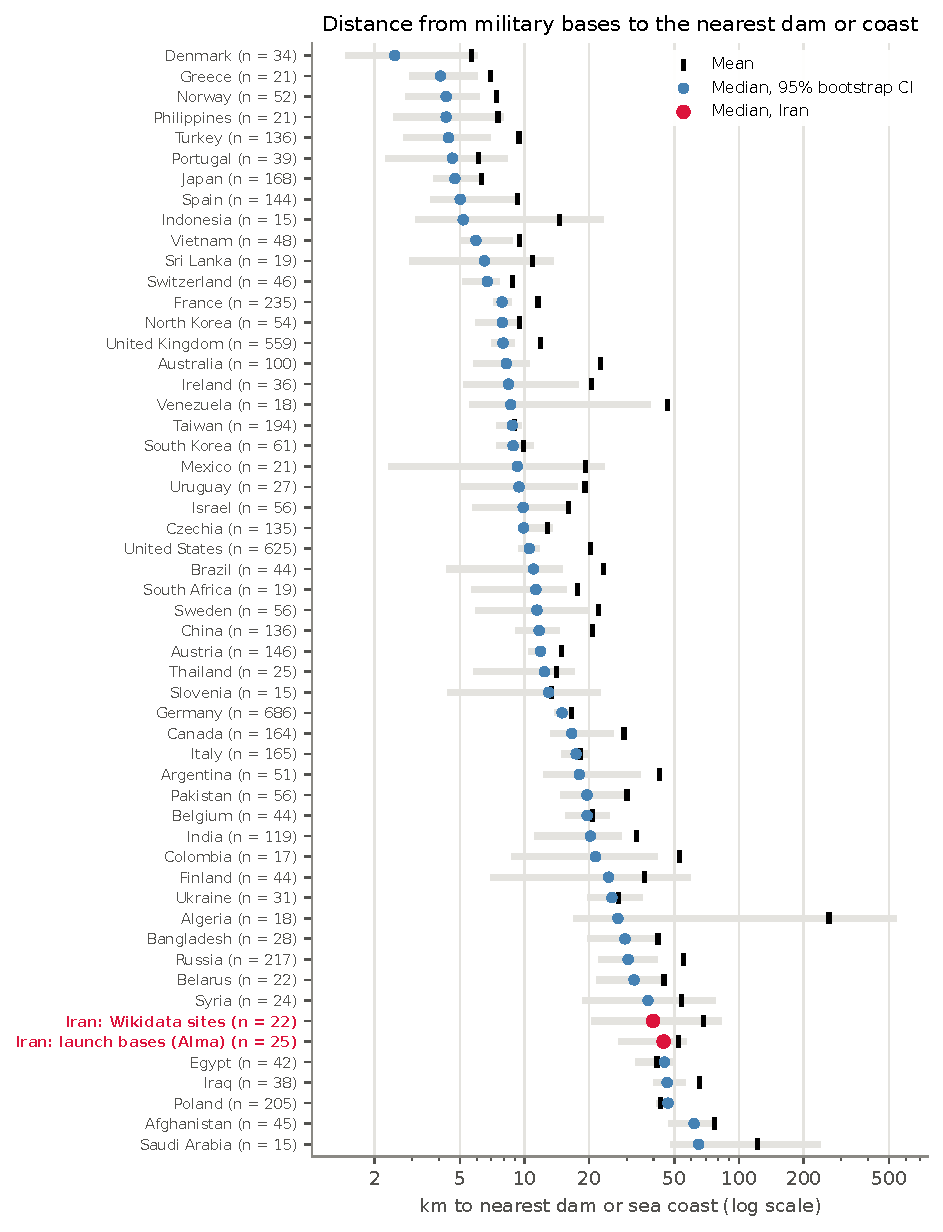
\includegraphics[width=\linewidth]{figures/fig7_rank_water.pdf}
\caption{Median (with 95\% bootstrap interval) and mean distance from military sites to the nearest dam or sea coast, by country. Iranian rows are shown in crimson: the launch bases and the 22 Iranian sites recorded in Wikidata.}
\label{fig:rank}
\end{figure}

The Iranian launch bases have a median distance to the nearest dam or coast of \AlmaWater{}~km, which ranks \RankWater{}th of \RankOf{}; military sites in \ShareCloser\% of the ranked countries lie closer to water (Figure~\ref{fig:rank}, Table~\ref{tab:rank}). For dams alone the Iranian launch bases rank \RankDam{}th. Relative to Iran's own geography (ratio \AlmaWaterRatio{}), they rank \RankWaterRatio{}th for dams or coast and \RankDamRatio{}th for dams, close to the median of the distribution. Military sites in Turkey, Spain, Japan, France, the United Kingdom, the United States and China all lie closer to dams than the Iranian launch bases do (Figure~\ref{fig:rankdam}).

\paragraph{Caveats.} Wikidata coverage is uneven: it records 686 German sites and 22 Iranian ones, and reflects what contributors have documented rather than an official inventory. GDW coverage of small dams also varies between countries; it records \NDams{} Iranian dams against the 533 reported in the NYT article, and 18 Saudi dams against an official count of 559. This undercount inflates Iran's absolute distances to dams, so the absolute dam ranking favours the argument made here. The ratio is the more appropriate comparison, because the random benchmark points within each country are subject to the same undercount. On that measure the Iranian launch bases are close to the median for dams and below the median for dams or coast. Neither result supports the view that Iranian military siting is unusually oriented towards water. The coastline component is unaffected by dam coverage.

\section{Dam construction as a response to water scarcity}
\label{sec:scarcity}
\begin{figure}[t]
\centering
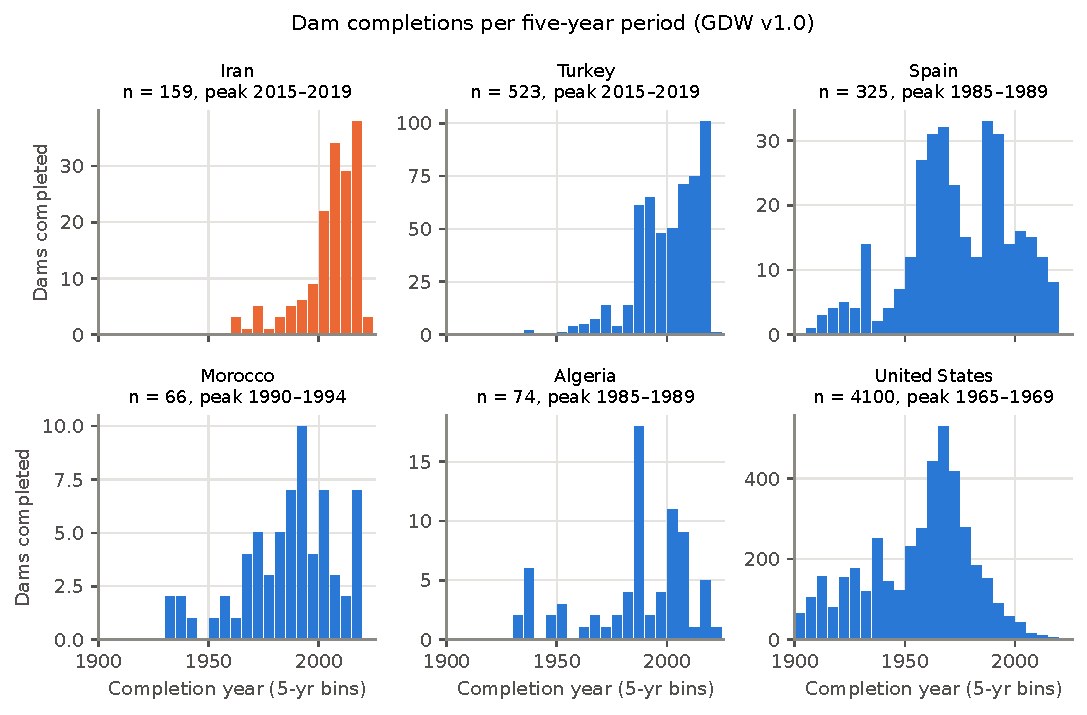
\includegraphics[width=\linewidth]{figures/fig5_timelines.pdf}
\caption{Dam completions per five-year period, GDW v1.0 (dams with a recorded completion year). The final Iranian bin covers 2020--2021 only.}
\label{fig:timelines}
\end{figure}
\begin{figure}[t]
\centering
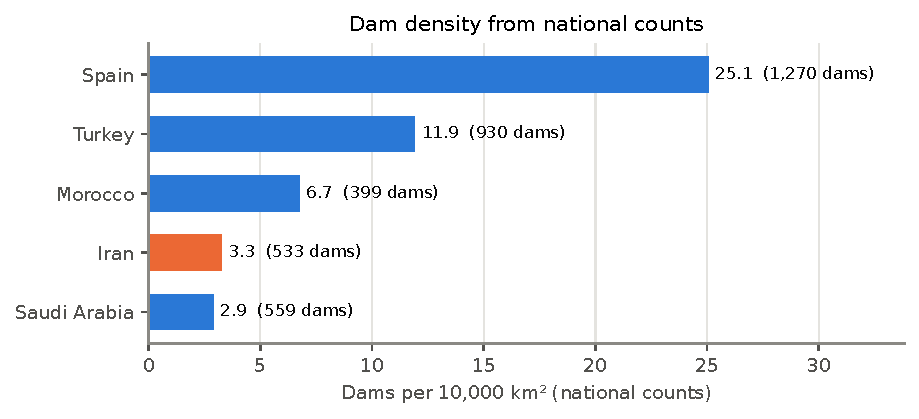
\includegraphics[width=\linewidth]{figures/fig6_density.pdf}
\caption{Dams per 10,000~km$^2$ from national counts: Iran (533, as reported in the NYT article), Turkey \citep{rew_turkey}, Spain \citep{berga2006spain}, Morocco \citep{mipa_morocco} and Saudi Arabia \citep{saudipedia_dams}. Definitions differ: Spain's figure counts large dams only, whereas Iran's includes small dams, so the comparison if anything overstates Iran's relative density.}
\label{fig:density}
\end{figure}

Semi-arid states with the necessary resources have commonly responded to water scarcity by building dams. Spain built some 1,270 large dams, more than any other European country \citep{berga2006spain}. In 1967 King Hassan II of Morocco launched the \emph{politique des barrages} with the aim of irrigating one million hectares; the number of Moroccan dams rose from 13 at independence to more than 100 \citep{mwn_morocco}, and the country now has 144 large dams and 255 hill dams \citep{mipa_morocco}. Saudi Arabia, which has no permanent rivers, operates 559 dams \citep{saudipedia_dams} and plans a further 1,000. Turkey has 930 \citep{rew_turkey}.

Iran's programme is late rather than anomalous. Of its dams with a recorded completion year, \IranAfterNinety\% were completed after 1990, with a peak in \IranTLpeak--\the\numexpr\IranTLpeak+4\relax{}. Turkey's programme peaks in the same period (\TurAfterNinety\% after 1990; peak \TurTLpeak--\the\numexpr\TurTLpeak+4\relax{}; Figure~\ref{fig:timelines}). The 533 Iranian dams reported in the NYT article correspond to 3.3 per 10,000~km$^2$, fewer than in Spain, Turkey or Morocco (Figure~\ref{fig:density}).

Where individual Iranian dams lack an evident civilian rationale, a documented civilian explanation is available in the political economy of construction. The IRGC's construction conglomerate, Khatam al-Anbiya, is reported to have built 25 of Iran's 45 billion cubic metres of storage capacity \citep{rudaw_kaa}, and analysts describe a ``water mafia'' with a durable claim on the national budget \citep{mei_watermafia}. One of the NYT article's two authors has previously made this case: \citet{dawn_madani} attributed Iran's water crisis in part to the government's ``excessive construction of dams and water transfer tunnels'' over many years. Patronage and mismanagement can account for dams without a clear purpose without reference to missile programmes. It should nonetheless be acknowledged that the same conglomerate also builds tunnels for the armed forces; this is the strongest point in favour of the NYT article's hypothesis.

\section{Legal significance of the NYT article's framing}
\label{sec:law}
Under Additional Protocol~I, dams may not be attacked, even when they constitute military objectives, if the attack may release dangerous forces and cause severe losses among the civilian population. Their special protection ceases only if a dam is used ``for other than its normal function'' and in regular, significant and direct support of military operations \citep{apI}. Iran and the United States signed the Protocol but have not ratified it \citep{unprotocols}, so customary law governs between them \citep{lieber2022dams}; under the customary rule, ``particular care must be taken'' when attacking dams and installations in their vicinity \citep{icrcrule42}. A public account, such as the NYT article, that recasts civilian dams as military supply infrastructure weakens that protection in practice, in a conflict in which US strikes have already damaged Iranian drinking-water reservoirs. A claim with these consequences should meet a high evidential standard. The analysis above indicates that the NYT article's claim does not meet it.

\section{Evidential weaknesses of the NYT article}
\label{sec:weak}
Beyond the statistical results, three features of the NYT article's evidence deserve note.
\begin{enumerate}
\item \textbf{Absence of a quantitative test.} The agreement of the seven experts quoted in the NYT article and a visual match between two maps do not establish co-location beyond chance. Section~\ref{sec:test} shows that the apparent association disappears under standard controls.
\item \textbf{Balance of sources.} The security analysts quoted are a former Israeli military intelligence analyst and a fellow of the Washington Institute; the only Iranian official named in the excerpts available to us is a member of parliament.
\item \textbf{Relationship with the principal source.} One of the NYT article's two authors has co-written at least two pieces with Nima Shokri, whose dam map is the NYT article's central evidence \citep{conversation_mahoozi_shokri}. We could not confirm from the available excerpts whether the NYT article discloses this.
\end{enumerate}

\section{Limitations}
\begin{itemize}
\item The NYT article's full text, Shokri's dam map and the NYT article's strike map were not available; we used the closest public substitutes. The conclusions should be re-examined if those data are released.
\item Terrain is represented at 10$'$ (about 18~km), which is coarse; most of the adjustment comes from matching on towns and rivers. Finer terrain data would refine M1 but are unlikely to change the result under M3.
\item Twenty-five bases is a small sample; the intervals in Table~\ref{tab:nulls} reflect this.
\end{itemize}

\section*{Data and code availability}
All data, code and figures are available at \url{https://github.com/osolari/iran-dams-colocation}, with documentation at \url{https://osolari.github.io/iran-dams-colocation}. Every number and table in this report is generated by the code from the data; none is transcribed by hand. The full analysis, including this document, is reproduced by running \texttt{run\_all.sh}.

\bibliographystyle{plainnat}
\bibliography{shared/bibliography/references}

\postauthorcard

\clearpage
\appendix
\section{Launch bases and nearest dams}
\footnotesize
\begin{longtable}{@{}rlrrcp{4.2cm}r@{}}
\toprule
\# & Base & Lat & Lon & Struck 2025 & Nearest dam (GDW) & km \\
\midrule\endhead
\inputtable{tab_bases.tex}
\bottomrule
\end{longtable}

\section{Country ranking}
\footnotesize\setlength{\tabcolsep}{4pt}
\begin{longtable}{@{}rp{4.2cm}rrrrrr@{}}
\caption{Distances (km) from military bases to water by country. Water = nearest dam or sea coast. Ratio = median for bases / median for random points in the same country.}\label{tab:rank}\\
\toprule
Rank & Country & $n$ & \multicolumn{2}{c}{Water} & Dam & Coast & Ratio \\
 & & & median & mean & median & median & \\
\midrule\endfirsthead
\toprule
Rank & Country & $n$ & \multicolumn{2}{c}{Water} & Dam & Coast & Ratio \\
 & & & median & mean & median & median & \\
\midrule\endhead
\inputtable{tab_ranking.tex}
\bottomrule
\end{longtable}

\begin{figure}[h]
\centering
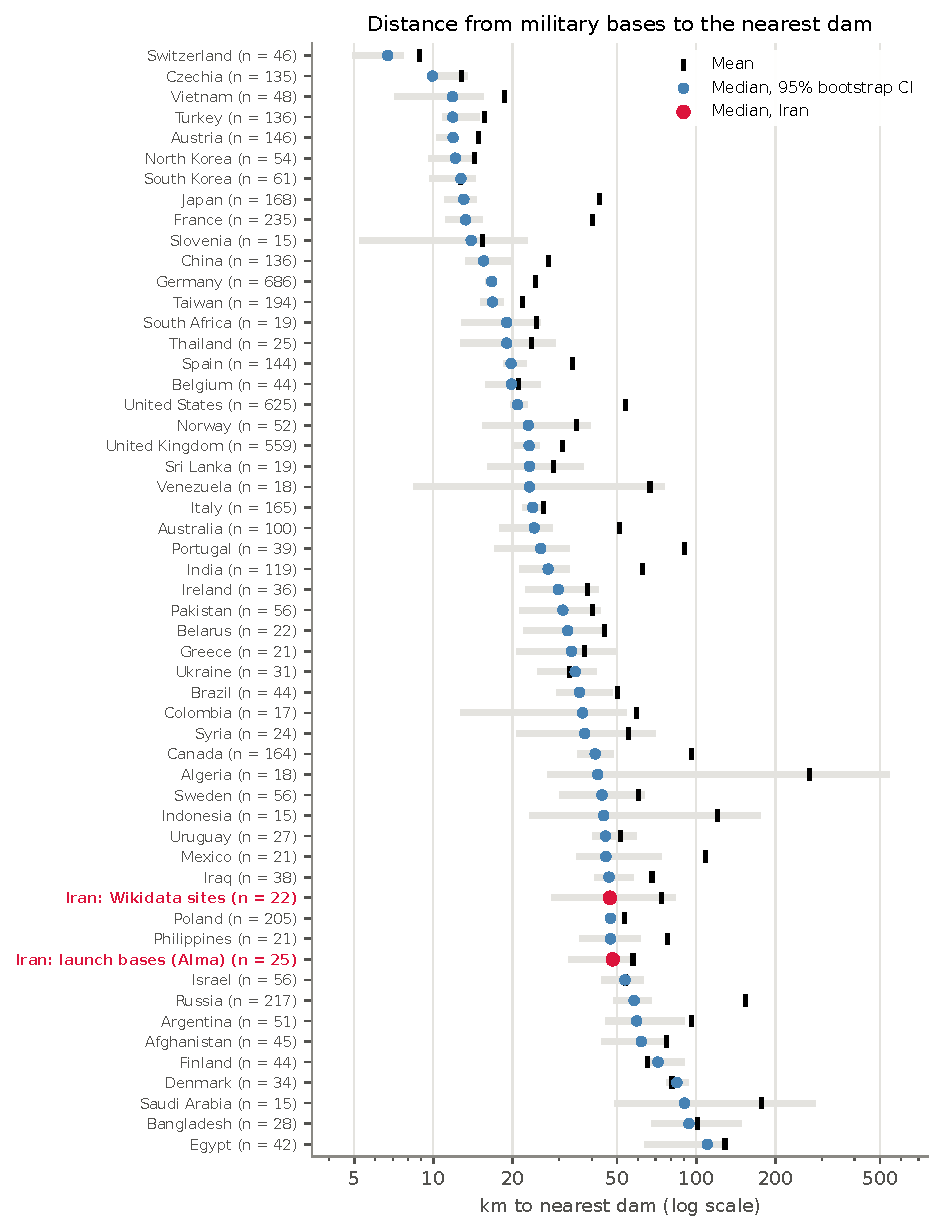
\includegraphics[width=\linewidth]{figures/fig8_rank_dam.pdf}
\caption{As Figure~\ref{fig:rank}, dams only.}
\label{fig:rankdam}
\end{figure}

\end{document}
